\documentclass[12pt,addpoints]{exam}
%\usepackage{enumitem}
\usepackage{amsfonts,amssymb,amsmath, amsthm}
\usepackage{graphicx}
\usepackage{systeme}
\usepackage{pgf,tikz,pgfplots}
\pgfplotsset{compat=1.15}
\usepgfplotslibrary{fillbetween}
\usepackage{mathrsfs}
\usetikzlibrary{arrows}
\usetikzlibrary{calc}
\usepackage{geometry}
\geometry{
	a4paper,
	total={170mm,257mm},
	left=20mm,
	top=20mm,
}
\date{October, 2023}
\pagestyle{headandfoot}
%\firstpageheadrule
\runningheader{Vectors}{}{Page \thepage\ of \numpages}
\runningheadrule
\firstpagefooter{}{}{}
\runningfooter{By Aaron G.K.}{}{Page \thepage\ of \numpages}
\title{Vectors}
\author{Aaron G.K.}
\begin{document}
	\maketitle
	Vectors are essential to physics and engineering. Many fundamental physical quantities are vectors, including displacement, velocity, force, and electric and magnetic vector fields. Scalar products of vectors define other fundamental scalar physical quantities, such as energy. Vector products of vectors define still other fundamental vector physical quantities, such as torque and angular momentum. In other words, vectors are a component part of physics in much the same way as sentences are a component part of literature.
	\subsection*{Scalars and Vectors}
    Many physical quantities can be specified completely by giving a single number and the appropriate unit. For example, “a class period lasts 50 min” or “the gas tank in my car holds 65 L” or “the distance between two posts is 100 m.” A physical quantity that can be specified completely in this manner is called a scalar quantity. Scalar is a synonym of “number.” Time, mass, distance, length, volume, temperature, and energy are examples of scalar quantities.
    \\ \\
    Some other physical quantities, however, cannot be described completely by just a single number of physical units - they may need a direction attached to the scalar to give it the full meaning. Physical quantities specified completely by giving a number of units (magnitude) and a direction are called vector quantities. 
    \subsection*{Representation of Vectors}
    \begin{center}
    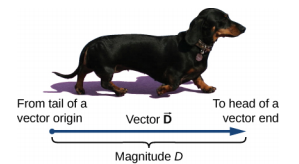
\includegraphics[scale=0.5]{dog.png}	
    \end{center}
    We draw a vector from the initial point or origin (called the \textbf{tail}) to the end or terminal point (called the \textbf{head}), marked by an arrowhead. Magnitude is the length of a vector and is \textbf{always a positive }scalar quantity. \\ \\
    To see how vectors work, let's take a simple displacement vector shown in the figure below.
    \begin{center}
    	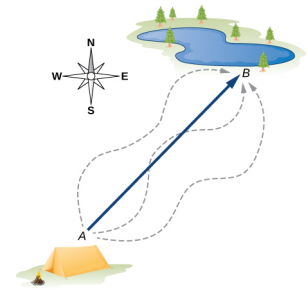
\includegraphics[scale=0.4]{disp.png}
    \end{center}
    The displacement vector from point A to point B is indicated by an arrow with origin at point A and end at point B. The displacement is the same for any of the actual paths (dashed curves) that may be taken between points A and B. \\ \\
    Two vectors that have identical directions are said to be parallel vectors—meaning, they are parallel to each other. Two parallel vectors $\vec{A}$ and $\vec{B}$ are equal, denoted by $\vec{A}=\vec{B}$, if and only if they have equal magnitudes $\vec{A}=\vec{B}$. Two vectors with directions perpendicular to each other are said to be orthogonal/perpendicular vectors. 
    \begin{center}
    	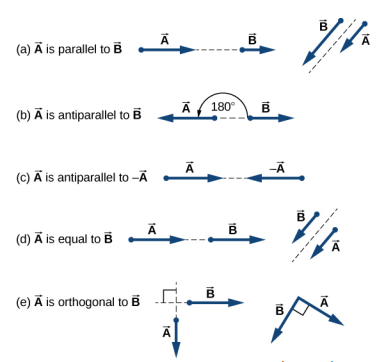
\includegraphics[scale=0.6]{vectors.png}
    \end{center}
    \subsection*{Algebra of Vectors}
    In a vector equation, both sides of the equation are vectors. In general, when a vector $\vec{A}$ is multiplied by a positive scalar $\alpha$, the result is a new vector $\vec{B}$
    that is parallel to $\vec{A}$. The magnitude the new vector($\vec{B}$) is obtained by multiplying the magnitude of the original vector($\vec{A}$) with the scalar.
    $$\vec{B} = \alpha \vec{A}\hspace{1cm}\text{\&}\hspace{1cm}|\vec{B}|= |\alpha| |\vec{A}|$$
    Based on the scalar we multiply the original vector with, we can change the following aspects of the vector
    \begin{itemize}
    	\item if $|\alpha|>1$, the magnitude of the new vector will be larger 
    	\item if $|\alpha|>1$, the magnitude of the new vector will be smaller
    	\item if $\alpha>0$, the new vector will be parallel to the original vector
    	\item if $\alpha<0$, the new vector will be anti-parallel to the original vector
    \end{itemize}
	Most of the applications of vectors lies in operations on vectors. One significant operation is addition of vectors. The sum of vectors is called the resultant. 
	$$\vec{R}=\vec{A}+\vec{B}$$
	For vectors that act along one dimension, it is as simple as adding/subtracting their magnitudes depending on whether they are parallel or anti-parallel. 
	\\ \\
	When adding many vectors in one dimension, it is convenient to use the concept of a unit vector. A unit vector, which is denoted by a letter symbol with a hat, such as  $\hat{v}$, has a magnitude of one and does not have any physical unit. The only role of a unit vector is to specify direction.
	$$\hat{v}=\dfrac{\vec{v}}{|\vec{v}|}$$
	Vector addition has a few of these properties:
	\begin{itemize}
		\item Commutativity $\vec{A} + \vec{B} = \vec{B} + \vec{A}$
		\item Associativity $(\vec{A} + \vec{B}) + \vec{C} = \vec{A} + (\vec{B} + \vec{C})$
		\item Distributive over scalars $\alpha_{1} \vec{A} + \alpha_{2} \vec{A} = (\alpha_{1} + \alpha_{2}) \vec{A}$
	\end{itemize}
	However, when dealing with multi-dimensional(two \& more), we have to have a bit more complicated process to come up at out resultant. One simple way of adding these vectors is using a graphical addition method. The two common ones are the parallelogram method and the more popular, triangle method.
	\subsubsection*{Parallelogram Method}
	Make the parallel translation of each vector to a point where their origins (marked by the dot) coincide and construct a parallelogram with two sides on the vectors and the other two sides (indicated by dashed lines) parallel to the vectors. 
	\begin{center}
		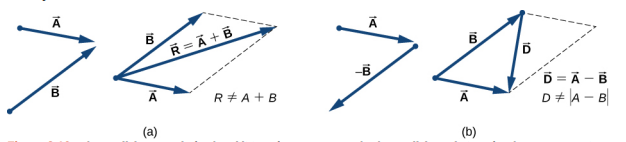
\includegraphics[scale=0.5]{parallelogram.png}
	\end{center}
	\begin{itemize}
		\item $\vec{A}+\vec{B}$ Draw the resultant vector $\vec{R}$ along the diagonal of the parallelogram from the common point to the opposite corner. \textit{\textbf{Length R of the resultant vector is not equal to the sum of the magnitudes of the two vectors}}.
		\item $\vec{A}-\vec{B}$ Draw the difference vector $\vec{D}$ along the diagonal connecting the ends of the vectors. Place the origin of vector $\vec{D}$ at the end of vector $\vec{B}$ and the end of vector $\vec{D}$ at the end of vector $\vec{A}$. \textit{\textbf{Length D of the difference vector is not equal to the difference of magnitudes of the two vectors.}} 
	\end{itemize} 
	\subsubsection*{Triangle Method}
	 Suppose we want to draw the resultant vector of the four vectors shown below. We select any one of the vectors as the first vector and make a parallel translation of a second vector to a position where the tail of the second vector coincides with the head of the first vector. Then, we select a third vector and make a parallel translation of the third vector to a position where the tail of the third vector coincides with the head of the second vector. We repeat this procedure until all the vectors are in a head-to-tail arrangement as shown below.
	\begin{center}
		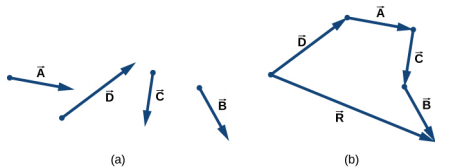
\includegraphics[scale=0.5]{triangle.png}
	\end{center}
	The resultant vector is drawn from the tail of the first vector to the head of the last vector in this arrangement.
	\subsubsection*{Analytical Methods}
	For daily applications and numerical implementations of vectors, graphical addition doesn't seem to be atop of the options. We would rather use actual defined algebraic representation of vectors which can be implemented through coordinate systems. \\ \\
	For a simple two dimensional vector, the vector is described by a pair of its vector coordinates. Consider the vector below on the Cartesian plane.
	\begin{center}
		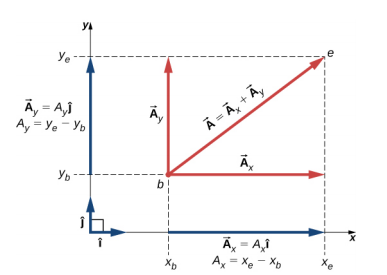
\includegraphics[scale=0.6]{2d.png}
	\end{center}
	Following the parallelogram rule for vector addition, each vector on a Cartesian plane can be expressed as the vector sum of its vector components
	$$\vec{A} = \vec{A}_{x} + \vec{A}_{y}$$
	We usually denote the positive direction on the x-axis by the unit vector $\hat{i}$ and the positive direction on the y-axis by the unit vector $\hat{j}$. Unit vectors of the axes, $\hat{i}$ and $\hat{j}$, define two orthogonal directions in the plane. The x- and y- components of a vector can now be written in terms of the unit vectors of the axes:
	$$\begin{cases} \vec{A}_{x} = A_{x} \hat{i} \\ \vec{A}_{y} = A_{y} \hat{j} \end{cases}$$
	For a three dimensional version,
	$$\begin{cases} \vec{A}_{x} = A_{x} \hat{i} \\ \vec{A}_{y} = A_{y} \hat{j} \\ \vec{A}_{z} = A_{z} \hat{k} \end{cases}$$
	Thus, the vector can be expressed as
	$$\vec{A} = A_{x} \hat{i} + A_{y} \hat{j}$$\\
	For a three dimensional version,
	$$\vec{A} = A_{x} \hat{i} + A_{y} \hat{j} + A_{z} \hat{k}$$\\
	\subsection*{More on algebra of vectors}
	The generalization of the number zero to vector algebra is called the null vector, denoted by  $\vec{0}$. All components of the null vector are zero, $\vec{0}=0\hat{i}+0\hat{j}+0\hat{k}$, so the null vector has no length and no direction.\\ \\
	Based off of the definition above, two vectors $\vec{A}$ and $\vec{B}$ are equal vectors if and only if their difference is the null vector.
	$$\vec{0}=\vec{A}-\vec{B}=(A_x-B_x)\hat{i}+(A-y-B_y)\hat{j}+(A_z-B_z)\hat{k}=\vec{0}=0\hat{i}+0\hat{j}+0\hat{k}$$
	$$\vec{A} = \vec{B} \Leftrightarrow \begin{cases} A_{x} = B_{x} \\ A_{y} = B_{y} \\ A_{z} = B_{z} \end{cases}$$
	Hence, we can write  $\vec{A}=\vec{B}$ if and only if the corresponding components of vectors $\vec{A}$ and $\vec{B}$ are equal.
	\subsection*{Product of Vectors}
	A vector can be multiplied by another vector and there are two kinds of products of vectors used broadly in physics and engineering. One kind of multiplication is a scalar multiplication of two vectors. Taking a \textbf{scalar product} of two vectors results in a number (a scalar), as its name indicates. Scalar products are used to define work and energy relations. For example, the work that a force (a vector) performs on an object while causing its displacement (a vector) is defined as a scalar product of the force vector with the displacement vector. \\ \\ 
	A quite different kind of multiplication is a \textbf{vector multiplication} of vectors. Taking a vector product of two vectors returns as a result a vector, as its name suggests. Vector products are used to define other derived vector quantities. For example, in describing rotations, a vector quantity, torque is defined as a vector product of an applied force (a vector) and its lever arm (a vector). 
	\subsubsection*{Scalar Product}
	\begin{center}
		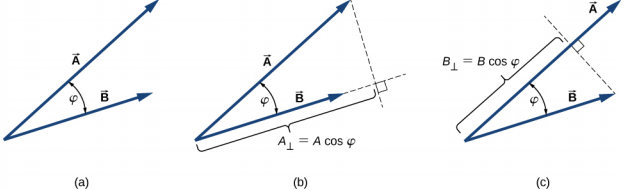
\includegraphics[scale=0.5]{dot.png}
	\end{center}
	The scalar product $\vec{A}\cdot\vec{B}$ of two vectors $\vec{A}$ and $\vec{B}$ is a number defined by the equation
	$$\vec{A}\; \cdotp \vec{B} = AB \cos \theta$$
	Where $\theta$ is the angle between the two vectors.\\ \\
	In the Cartesian coordinate system, scalar products of the unit vector of an axis with other unit vectors of axes always vanish because these unit vectors are orthogonal.
	$$\hat{i}\; \cdotp\; \hat{j} = |\hat{i}||\hat{j}| \cos 90^{o} = (1)(1)(0) = 0,$$
	$$\hat{i}\; \cdotp\; \hat{k} = |\hat{i}||\hat{k}| \cos 90^{o} = (1)(1)(0) = 0,$$
	$$\hat{k} \cdotp\; \hat{j} = |\hat{k}||\hat{j}| \cos 90^{o} = (1)(1)(0) = 0 $$
	Since the magnitude of all the unit vectors is 1, we also get
	$$\hat{i}\; \cdotp\; \hat{i} = i^{2} = \hat{j}\; \cdotp\; \hat{j} = j^{2} = \hat{k}\; \cdotp\; \hat{k} = 1$$
	As with the definition, we can portray the scalar product as the projection of the first vector over the other.
	$$\begin{cases} \vec{A}\; \cdotp \vec{B}  = AB \cos \theta \\ \vec{A}\; \cdotp \vec{B} = B(A \cos \theta) = BA_{\parallel} \\ \vec{A}\; \cdotp \vec{B} = A(B \cos \theta) = AB_{\parallel} \ldotp \end{cases}$$
	For example, in the Cartesian coordinate system in a plane, the scalar x-component of a vector is its dot product with the unit vector $\hat{i}$, and the scalar y-component of a vector is its dot product with the unit vector $\hat{j}$:
	$$\begin{cases} \vec{A}\; \cdotp\; \hat{i} = |\vec{A}||\hat{i}| \cos \theta_{A} = A \cos \theta_{A} = A \cos \theta_{A} = A_{x} \\ \vec{A}\; \cdotp\; \hat{j} = |\vec{A}||\hat{j}| \cos (90^{o} - \theta_{A}) = A \sin \theta_{A} = A_{y} \end{cases}$$
	To compute the scalar product of two vectors when they're in their component forms, we can do this. Consider two vectors shown below
	$$\vec{A} = A_{x}\; \hat{i} + A_{y}\; \hat{j} + A_{z}\; \hat{k}\; \text{ and } \vec{B} = B_{x}\; \hat{i} + B_{y}\; \hat{j} + B_{z}\; \hat{k},$$
	The scalar product is defined as
	$$\begin{cases} \vec{A}\; \cdotp \vec{B}  = (A_{x}\; \hat{i} + A_{y}\; \hat{j} + A_{z}\; \hat{k})\; \cdotp (B_{x}\; \hat{i} + B_{y}\; \hat{j} + B_{z}\; \hat{k}) \\  = A_{x}B_{x}\; \hat{i}\; \cdotp\; \hat{i} + A_{x}B_{y}\; \hat{i}\; \cdotp\; \hat{j} + A_{x}B_{z}\; \hat{i}\; \cdotp\; \hat{k} \\  + A_{y}B_{x}\; \hat{j} \cdotp\; \hat{i} + A_{y}B_{y}\; \hat{j}\; \cdotp\; \hat{j} + A_{y}B_{z}\; \hat{j} \cdotp\; \hat{k} \\  + A_{z}B_{x}\; \hat{k}\; \cdotp\; \hat{i} + A_{z}B_{y}\; \hat{k}\; \cdotp\; \hat{j} + A_{z}B_{z}\; \hat{k}\; \cdotp\; \hat{k} \ldotp \end{cases}$$
	The above product simplifies to the answer below
	$$\vec{A}\; \cdotp \vec{B} = A_{x}B_{x} + A_{y}B_{y} + A_{z}B_{z}$$
	\subsubsection*{Vector Product}
	\begin{center}
		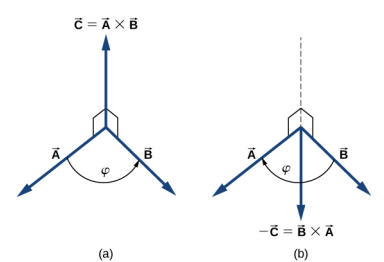
\includegraphics[scale=0.5]{cross.png}
	\end{center}
	 The vector product of two vectors $\vec{A}$ and $\vec{B}$ is denoted by $\vec{A}\times\vec{B}$ and is often referred to as a cross product. The vector product is a vector that has its direction perpendicular to both vectors  $\vec{A}$ and $\vec{B}$. In other words, vector $\vec{A}\times\vec{B}$ is perpendicular to the plane that contains vectors $\vec{A}$ and $\vec{B}$. The magnitude of the vector product is defined as
	 $$|\vec{A} \times \vec{B}| = AB \sin \theta$$
	 In another way, we can define the vector $\vec{A}\times\vec{B}$ as follows
	 $$\vec{A}\times\vec{B}=AB \sin \theta \hat{n}$$
	 Where $\hat{n}$ is a unit vector perpendicular to the plane that contains vectors $\vec{A}$ and $\vec{B}$. \\ \\
	 Unlike scalar product, the vector product is not commutative. In fact, it is anti-commutative:
	 $$\vec{A} \times \vec{B} = - \vec{B} \times \vec{A} $$
	 Similar to the dot product, the cross product has the following distributive property:
	 $$\vec{A} \times (\vec{B} + \vec{C}) = \vec{A} \times \vec{B} + \vec{A} \times \vec{C}$$
	 As we did with the scalar product, let's do the vector product with the component form of vectors. The most visible one is
	 $$\hat{i} \times \hat{i} = \hat{j} \times \hat{j} = \hat{k} \times \hat{k} = 0$$
\end{document}	